To evaluate our proposed module system we carried out a case study where
the JastAdd Extensible Java Compiler (JastAddJ), a system entirely based on
inter-type declarations, was retrofitted to use modules. JastAddJ is a
modular Java compiler designed particularly with extensibility in mind,
that uses ITDs and attribute grammars as its main modularization
mechanisms.  We have previously reported on the merits of this combination
in \cite{aosd08abc}. However, there are some nuisances related to using
multiple variants in the same system and certain properties with
unnecessary global scope that makes it a prime target for our proposed
module system. 

We believe this application serves as a suitable case to study when
evaluating the merits of the module system on realistic examples for
several reasons: 1) It is a reasonably sized application of more than
21,000 lines of code not counting documentation and white space.  3) It is
designed using ITDs from the beginning, completely separating behavior
from the class hierarchy using the paradigm that "everything is an ITD". 2)
The system is commonly used in various applications requiring extensible
compiler frontends, e.g., the Soot bytecode manipulation framework, and the
AspectBench Compiler.

\subsection{JastAdd Java Compiler Overview}
\label{jastaddjoverview}
The compiler consists of four main components: a \emph{Java 1.4 frontend}
with a corresponding \emph{Bytecode backend}, a \emph{Java 5 frontend} with
a \emph{Bytecode backend} as illustrated by Figure~\ref{MainComponents}. 

\begin{figure}[htb!]
  \begin{center}
    \resizebox{8.5cm}{!}{
      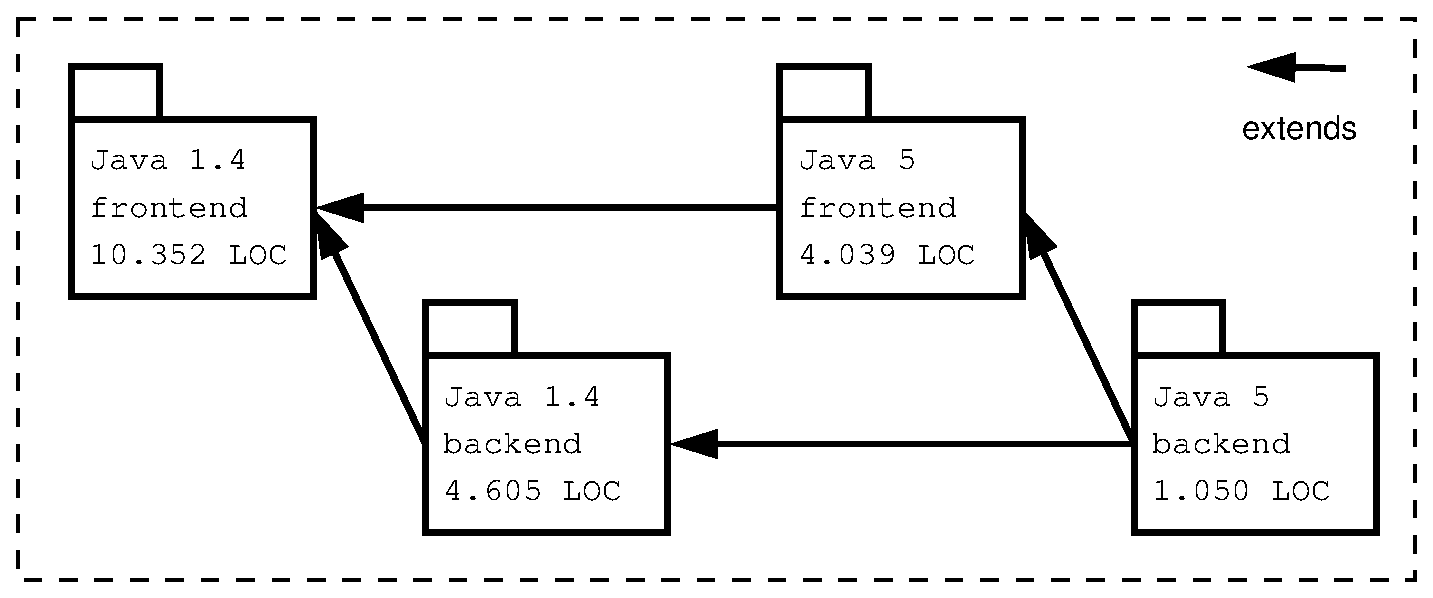
\includegraphics{figures/MainComponents}
    }
    \caption{The main components of JastAddJ}
    \label{MainComponents}
  \end{center}
\end{figure}

The components themselves are composed of AST "`base"' classes, and the
aspects that introduce the ITDs to the said classes. The AST classes
directly or indirectly extend the classes \texttt{ASTNode}, \texttt{List}, and \texttt{Opt},
which form the JastAdd framework classes. 

Since there is no module system each component is represented as a
directory of reusable source files that are combined using build files. The
Java 5 frontend is an extension to the Java 1.4 frontend, reusing its
source file, while specifying Java 5 language features as an increment to
the Java 1.4 frontend. A build file to create a Java 1.4 semantic checker
will thus only include files from the Java 1.4 folder, while a build file
for a Java 5 semantic checker includes files from both folders. The
backends are extensions to the frontends and reuse source files in a
similar manner.  By changing which files to include in the build it is
possible to build four different tools from these components.

Each frontend can be further divided into the following subcomponents: a
parser that builds an AST, a bytecode reader that reads class files, and a
semantic analyzer or code generator. The parser is generated from a context
free grammar, the bytecode reader is written in plain Java, and the
analyzers and code generators are implemented using attribute grammars and
inter-type declarations.

The architecture has a few problems that can be elegantly solved using a
module system. First, the different variants of the compiler can not
coexist in the same system since ITDs destructively update the class
hierarchy. This is handled with an ugly hack where multiple build files and
scripts are used generate compilers to different packages.  Second, the
bytecode readers are implemented in plain Java in a fashion which
unfortunately makes them quite hard to extend and we therefore use
different implementations of the reader in the Java 1.4 frontend and the
Java 5 frontend. This is handled by including different versions of source
files in the build for the Java 5 frontend and excluding some of the files
in the Java 1.4 frontend. Third, the systems are composed into one global
namespace which is terrible from an information hiding point of view.

\subsection{Applying Modules}

To remedy the problems detailed above, we apply the module system to
the JastAddJ compiler. We have refactored the components such that:

\begin{enumerate}
\item {The JastAdd framework classes reside in their own module.}
\item {The AST classes in the frontend components have been separated from the aspects, and extend the JastAdd framework module.}
\item {The Java 1.5 frontend extends the 1.4 frontend, and similarly with the backends and the AST modules}
\item {Dependencies between the modules were explicitly defined by the use of imports in the module declarations.}
	
\end{enumerate}

\begin{figure}[htb!]
  \begin{center}
    \resizebox{3in}{!}{
      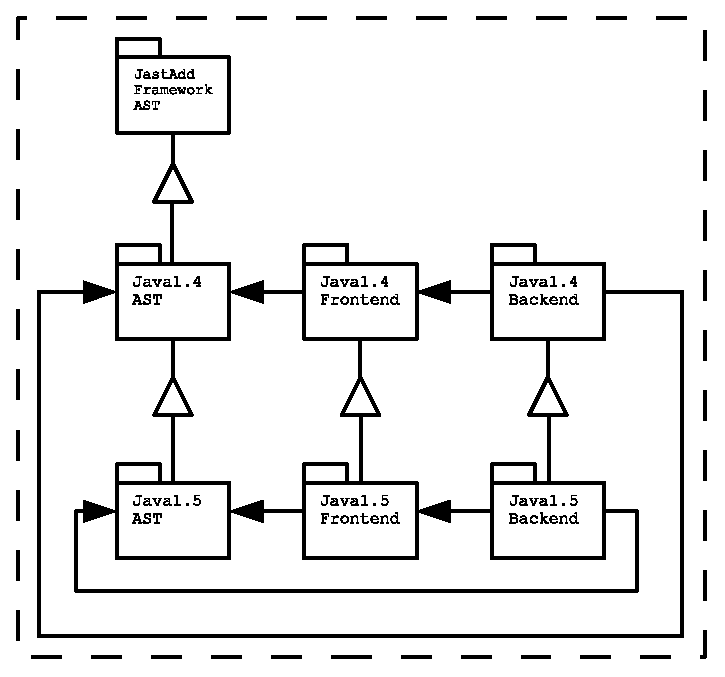
\includegraphics{figures/ModuleMainComponents}
    }
    \caption{JastAddJ refactored to use modules}
    \label{ModuleMainComponents}
  \end{center}
\end{figure}

Other than the necessary changes to use modules, it was also necessary to change the 
access modifiers of several ITDs from package private to public, to allow the 
access of these ITDs from outside their module. 

An example compiler application that uses the JastAddJ with modules is shown in the example below.
The module for the compiler application imports a frontend and a backend, and since the backend 
also imports an instance of the frontend, the \texttt{javacompiler} module contains a merge
operation that allows the java compiler and the backend to share the frontend classes.

\begin{lstlisting}[caption={JastAddJ Compiler Application}]
//file javacompiler.module
module javacompiler;
import own java15frontend as frontend;
import own java15backend as backend;
//merge the frontends to point to the same instance
merge frontend, backend::frontend as java15frontend frontend;
\end{lstlisting}

\subsection{Evaluation}

%Shows dependencies explicitly, information hiding, enables sharing through merge
The addition of modules to JastAddJ has made the dependencies of the components
explicit, and will lessen the chance of inadvertently introducing dependencies 
in the future. 

%everything used to be globally visible
%  modules improves information hiding 
%    (concrete example would be nice)
%    percent that became non-global
Information hiding among the components of the system has also benefited from
the introduction of modules. In the previous system, the class files produced from
compilation all belong to the same package, which means that a package private access modifier
is equivalent to a public modifier. Though several ITDs needed to be changed from 
package private to public to allow access from outside, a great majority remained private to
the module. As an example, in the Java 1.4 frontend, 24 ITDs (including synthesized attributes)
were changed from package private to public to allow other modules to access them. This is a small number 
compared to the total number of synthesized attributes alone (541) that were package private in the pre-module version.
This has effectively reduced the public ITD signature of the the Java 1.4 frontend to 5\% of its previous state.

%enables variants with different sets of ITDs
%  examples
The module system also allows instances of the frontend and backend with different versions
to exist in the same system, albeit being unable to share types. This will prove to be useful
in an IDE application, where multiple versions of the frontend would be necessary to provide
as-you-type error checking to different source versions. The ability to instantiate the frontend
without also pulling in the backend will also reduce the size of the AST objects created, as the
ITDs introduced by the backend would not be present in the AST nodes of that instance.

%enables variants with replaced/overridden classes
%  example: bytecode reader
%  (reason, monolithic implementation not suitable for extension, therefore
%  replacement easier)
The use of aspect overriding has allowed the Java 1.5 bytecode parser aspects in the Java 1.5 frontend to
override the corresponding aspects in the Java 1.4 frontend without the build file hacks that involved
excluding the Java 1.4 bytecode parser files when building the 1.5 compiler. This demonstrates that
aspect overriding solves a problem that arises in a real aspect oriented system, as opposed to 
hypothetical examples.s


%can we characterize the typical changes needed?
%how intrusive/global were the changes?
The changes required to introduce modules into JastAddJ were minimal: just the addition of the module 
declarations in \texttt{.module} files, the module membership specifications in the existing compilation units,
and a change to the access modifiers of some ITDs to allow inter-access. Given the benefits of instantiation, 
module composition and information hiding, this is a relatively small price to pay.

%eliminate cycles as a side-effect
%  required by the module system
%  architecture improved/ should have been done that way from the beginning
%  in retrospect
The use of \textbf{own} module instances will also benefit the architecture of JastAddJ,
since cyclic dependencies that involve \textbf{own} instances will cause an error to
be raised by the compiler. This provides a compile-time architecture check to avoid cyclic dependencies,
and would allow the early detection of decisions that would have caused unnecessarily
tight coupling between the components.

%many properties
%are global even though a more local scope would improve information hiding.

%improve extensibility and information hiding



 
 
